\section{Proposed Neural Networks}
\label{sec:proposed_networks}

Varying neural backbones used to encode state information from observations for both actor and critic networks. 
In critic network, actions are concatenated by state information coming from backbones. 
Then, this concatenated vector is passed through feed forward layer with hyperbolic tangent activation then through a linear layer with single output. 
Before feeding observations to backbone, they are passed through a linear layer with 96 dimensional output. 
However, for only LSTM backbones, this layer is not used and observations are passed to LSTM backbone as it is. 
In actor network, backbone is followed by a single layer with tanh activation for action estimation. 
Again, observations are passed through a linear layer with 96 dimensional output, and this is not valid for LSTM.
Critic and Actor networks are illustrated in \figref{fig:nets} 

\begin{figure}
	\begin{subfigure}{.5\textwidth}
		\centering
		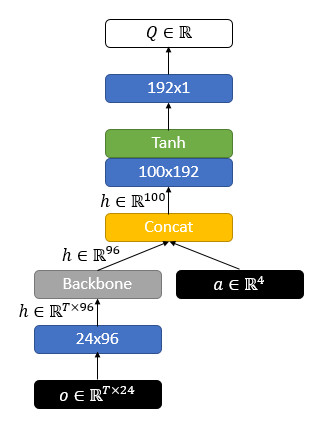
\includegraphics[width=0.97\linewidth]{figures/nets/critic.png}
		\caption{Critic Architecture}
		\label{fig:critic_net}
	\end{subfigure}
	\begin{subfigure}{.5\textwidth}
		\centering
		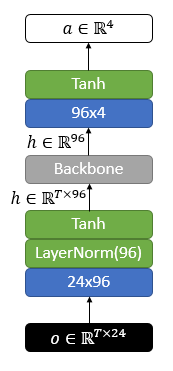
\includegraphics[width=0.55\linewidth]{figures/nets/actor.png}
		\caption{Actor Architecture}
		\label{fig:actor_net}
	\end{subfigure}
	\caption{Neural Architecture Design}
	\label{fig:nets}
\end{figure}

As backbones, following networks are proposed. 

\subsection{Residual Feed Forward Network}

Incoming vector is passed through 2 layers with 192 dimensional hidden size and 96 dimensional output with single skip connection, where there is GELU activation at first layer. 

\subsection{Long Short Term Memory}

Sequence of incoming vectors is passed though single vanilla LSTM layer with 96 dimensional hidden state. 
Output at last time step is considered as belief state. 

\subsection{Transformer (Pre-layer Normalized)}

Sequence of incoming vectors is passed through single pre-layer normalized transformer layer with 192 dimensional feed forward layer with GELU activation. 
In multi-head attention, 4 head is used and size of queries, keys and values are 8 for each head.
During multi-head attention, only the last observation is fed as query so that attentions are calculated only for last state.  
Its output is considered as belief state.
Note that excluding multi-head attention for this network gives our residual feed-forward neural network.
